\section{Unterteilungen und Minoren}

\textbf{Definition}: Sei $G=(V,E)$ ein Graph, $e=uv$ eine Kante. Dann ist die \textbf{Unterteilung von $\boldsymbol{e}$ in $\boldsymbol{G}$} der Graph $G\circ e=(V',E')$ mit
\begin{itemize}
	\item $V'=V+\{w\}$
	\item $E'=(E\setminus \{uv\})+\{uw,vw\}$
\end{itemize}
\bigskip
\textbf{Beobachtung}: $G$ planar $\iff$ $G\circ e$ planar\\

\textbf{Definition}: Graph $G$ ist eine \textbf{Unterteilung von $\boldsymbol{H}$} wenn $G=((H \circ e_1)\circ e_2)\cdots)\circ e_k$.
Wir sagen auch $G$ ist $\boldsymbol{H}$\textbf{-Unterteilung}.
Graph $G$ \textbf{enthält eine $\boldsymbol{H}$-Unterteilung}, wenn ein Teilgraph $G'\subseteq G$ eine $H$-Unterteilung ist.

\begin{center}
	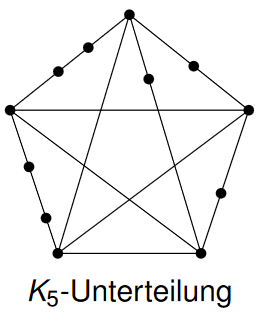
\includegraphics[width=0.17\textwidth]{images/k5-unterteilung.png}
\end{center}

\textbf{Beobachtung}: 
\begin{itemize}
	\item $K_5$- und $K_{3,3}$-Unterteilungen sind nicht-planar
	\item Jeder Graph der eine $K_5$ oder $K_{3,3}$-Unterteilung enthält, ist nicht planar
\end{itemize}
\bigskip
\textbf{Satz von Kuratowski}: $G$ ist planar $\iff$ $G$ enthält keine $K_5$- oder $K_{3,3}$-Unterteilung

\textit{Beweis}: \enquote{$\Rightarrow$} folgt aus obiger Beobachtung. Die Rückrichtung ist komplizierter und beweisen wir später.\\

\textbf{Definition}: Sei $G=(V,E)$ ein Graph, $e=uv$ eine Kante. Der Graph $G/e=(V',E')$ ist der Graph, der durch Kontrahieren der Kante $\boldsymbol{e}$ entsteht, genauer:
\begin{itemize}
	\item $V'=V\setminus\{u,v\}+\{w\}$
	\item $E'=E(G-u-v)\cup\{wa\mid au\in E \text{ oder } av\in E\}$
\end{itemize}
Diesen Prozess nennt man auch \textbf{Kantenkontraktion}. Dabei können Multikanten und Schlaufen entstehen.
\begin{center}
	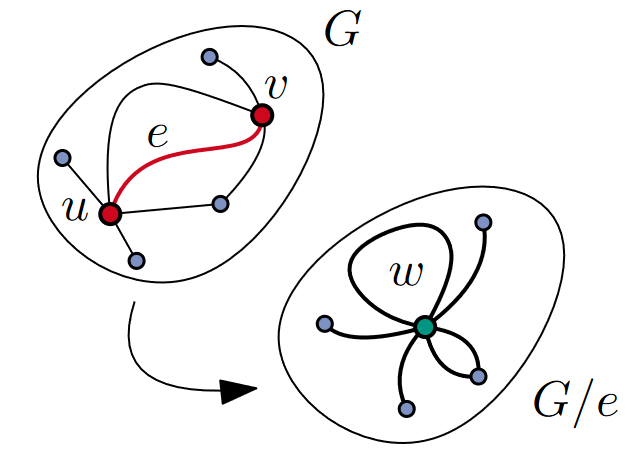
\includegraphics[width=0.3\textwidth]{images/kantenkontraktion.png}
\end{center}
\bigskip
\textbf{Definition}: Graph $H$ ist \textbf{Minor von} $\boldsymbol{G}$, wenn $H$ aus $G$ durch eine Folge von Kantenkontraktionen entsteht, also $H=((G/e_1)/e_2\cdots)/e_k$. Wir sagen dann auch: $G$ ist ein \textbf{$\boldsymbol{H}$-Minor} ($H$ ist der kleinere Graph, $G$ der Größere).\\

\textbf{Beobachtung}:
\begin{itemize}
	\item $G$ planar $\implies$ $G/e$ planar
	\item $G$ enthält $K_5$- oder $K_{3,3}$-Minor $\implies$ $G$ nicht planar
\end{itemize}
\bigskip
\textbf{Satz von Wagner}: $G$ planar $\iff$ $G$ enthält keinen $K_5$- oder $K_{3,3}$-Minor\\

\textbf{Lemma}: $G$ enthält $H$-Unterteilung $\implies $ $G$ enthält $H$-Minor

\textit{Beweis}: Kontrahiere durch Unterteilung entstandene Knoten zu ursprünglich adjazenten Knoten.
\begin{center}
	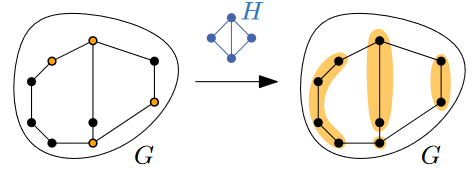
\includegraphics[width=0.35\textwidth]{images/um-skizze.png}
\end{center}
\pagebreak

\textbf{Es sind also äquivalent}:
\begin{enumerate}
	\item $G$ ist nicht planar
	\item $G$ enthält $K_5$- oder $K_{3,3}$-Minor
	\item $G$ enthält $K_5$- oder $K_{3,3}$-Unterteilung
\end{enumerate}

$(3)\implies(2)\implies(1)$ wurde schon bewiesen, $(1)\implies(2)\implies(3)$ müssen wir noch beweisen. Wir beginnen mit $(1)\implies(2)$.\\

\textit{Beweis von Wagner}: Es muss nur noch die Rückrichtung beweisen werden. Sei hierfür $G$ ein nicht-planarer Graph. Wir müssen einen $K_5$- oder $K_{3,3}$-Minor in $G$ finden. O.B.d.A. sei $G$ sogar minimal nicht-planar, d.h.
\begin{itemize}
	\item $G-v$ ist planar für jeden Knoten $v\in V$
	\item $G-e$ ist planar für jede Kante $e\in E$
	\item $G/e$ ist planar für jede Kante $e\in E$
\end{itemize}

Beweise zunächst folgendes Lemma:\\

\textbf{Lemma}: Sei $G$ minimal nicht-planar, $xy\in E(G)$. Dann ist $G-x-y$ ein Kreis.

\begin{wrapfigure}{r}{0.2\textwidth}
	\centering
	\vspace{30pt}
	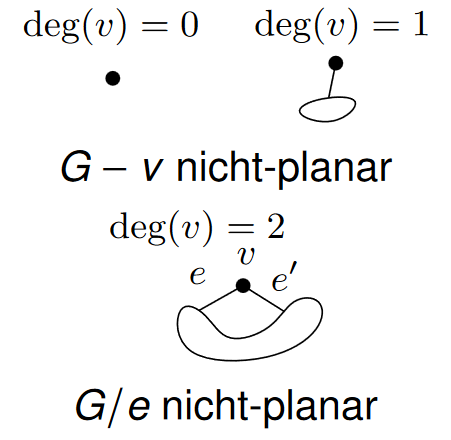
\includegraphics[width=0.22\textwidth]{images/wagner-1.png}
	\vspace{40pt}
	\vspace{-60pt}
\end{wrapfigure}
\textit{Beweis}: Da $G$ minimal nicht-planar ist,
\begin{itemize}
	\item ist $G$ zusammenhängend, da ansonsten Knoten aus einer Zusammenhangskomponente gelöscht werden könnte
	\item ist $\text{deg}(v)\geq 3$ für jeden Knoten $v\in V(G)$, denn Knoten von Grad 0 und 1 tragen nichts zur Nicht-Planarität bei, können also gelöscht werden ohne die Nicht-Planarität zu verlieren. Für einen Knoten $v$ von Grad 2 mit Kanten $e, e'$ bleibt $G/e$ nicht-planar. Wäre $G/e$ planar, so muss wegen $G = (G/e) \circ e'$ bereits $G$ planar sein. Widerspruch.
\end{itemize}

Das Lemma wird nun anhand von 3 Behauptungen bewiesen.

\underline{1. Behauptung}: $G-x-y$ enthält kein $\Theta$.

\textbf{Theta-Graphen} sind Unterteilungen des Graphen mit zwei Knoten und drei parallelen Kanten.
\begin{center}
	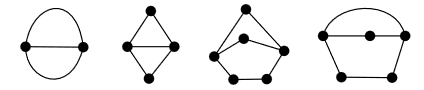
\includegraphics[width=0.3\textwidth]{images/theta.png}
\end{center}
\pagebreak


\textbf{Notation}: Für einen Kreis $C$ in einer planaren Zeichnung erhält man eine geschlossene \textbf{Jordankurve}, die die Ebene in zwei Komponenten unterteilt:
\begin{itemize}
	\item $\text{int}(C)$, das Innere von $C$
	\item $\text{ext}(C)$ , das Äußere von $C$
\end{itemize}
\begin{wrapfigure}{r}{0.25\textwidth}
	\centering
	\vspace{-70pt}
	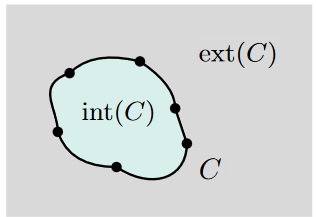
\includegraphics[width=0.22\textwidth]{images/jordan.png}
	\vspace{40pt}
	\vspace{-60pt}
\end{wrapfigure}

\textit{Beweis von Behauptung 1}:
\begin{itemize}
	\item Angenommen $G-x-y$ enthält ein $\Theta$.
	\item $G'\coloneqq G/xy$ ist planar mit Kante $xy$ zu Knoten $z$ kontrahiert.
	\item $G'-z=G-x-y$ ist ebenfalls planar.
	\item Zeichnung von $G'$ enthält ein $\Theta$ und das $\Theta$ hat 3 Kreise:
	\begin{center}
		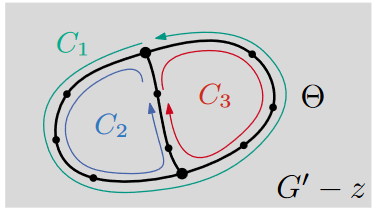
\includegraphics[width=0.3\textwidth]{images/wagner-2.png}
	\end{center}
	\item Betrachte Kreis $C$ im $\Theta$, sodass Knoten $z$ auf einer Seite von $C$ und eine Kante $e'\in E(\Theta)$ auf der anderen Seite von $C$ liegt.
	\item Wähle $\Theta$ und $C$ so, dass die Seite von $C$ mit $z$ inklusionsminimal ist, d.h. es gibt kein anderes $\Theta$ mit Kreis $C$, was $z$ enthält und ein kleineres Inneres hat
	\item O.B.d.A. gilt $z\in\text{int}(C)$ und $e'\in\text{ext}(C)$
	\begin{center}
		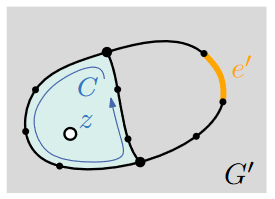
\includegraphics[width=0.27\textwidth]{images/wagner-3.png}
	\end{center}
	\item Betrachte $G''=G-\text{ext}(C)$.
	\item Da $e'\notin G''$ ist, wird mindestens eine Kante gelöscht, also ist $G''$ planar.
	\item Betrachte eine planare Zeichnung von $G''$ mit Kreis $C$.
\end{itemize}

\underline{Ziel}: Zeige, dass $C$ eine Facette berandet, denn dann kann $\text{ext}(C)$ in $C$ eingesetzt werden, was aber eine planare Zeichnung von $G$ wäre. \Lightning
\begin{center}
	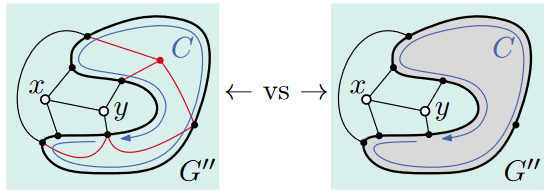
\includegraphics[width=0.4\textwidth]{images/wagner-4.png}
\end{center}

\begin{itemize}
	\item Betrachte Pfad $P$ in $G''$, der auf verschiedenen Knoten von $C$ startet und endet und ansonsten zu C disjunkt ist.
	\item $P$ entspricht auch einem Pfad $P'$ in $G'$.
\end{itemize}

Wenn $z\notin P'$:
\begin{itemize}
	\item Dann ist $C\cup P'$ ein $\Theta$ in $G-x-y$.
	\item Dieses $\Theta$ hat einen Kreis der $z$ enthält, aber ein kleineres Inneres als $C$ hat.
	\item Widerspruch zur Wahl von $\Theta$ und $C$.
\end{itemize}
\begin{center}
	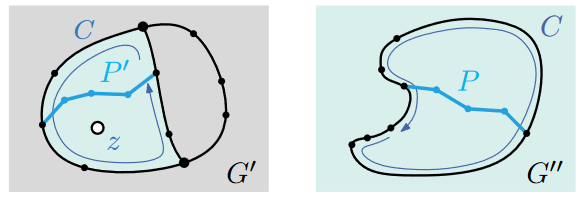
\includegraphics[width=0.4\textwidth]{images/wagner-5.png}
\end{center}

Also liegt $z$ auf $P'$ und $P$ muss $x$ oder $y$ enthalten. Also liegt jeder solche Pfad in der Zeichnung von $G''$ auf der Seite von $C$, die $xy$ enthält. 
\begin{center}
	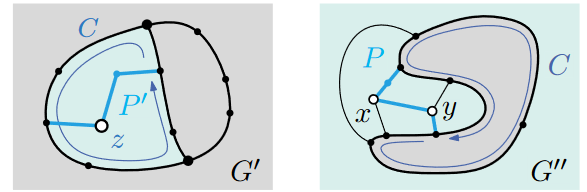
\includegraphics[width=0.42\textwidth]{images/wagner-6.png}
\end{center}

$\implies$ $C$ liegt im Rand einer Facette von $G''$

Damit ist \textit{Behauptung 1} bewiesen.

